\documentclass[border=2pt,tikz]{standalone}
\usetikzlibrary{shapes}

\newcommand{\ventil}[3]{%
    \draw (#1-1,#2-0.5) -- (#1+1,#2+0.5) -- (#1+1,#2-0.5) -- (#1-1,#2+0.5) -- cycle;
    \draw (#1,#2) -- (#1,#2-1);
    \draw (#1-0.3,#2-1) rectangle (#1+0.3,#2-1.5);
    \node at (#1,#2+1) {\bf #3};
}

\newcommand{\motor}[2]{
  \draw (#1,#2) circle(0.5cm);
  \node at (#1,#2) {\bf M};
}

\newcommand{\messung}[2]{
   \draw (#1,#2) circle (5mm);
   \draw [->] (#1-0.2,#2-0.3) -- (#1+0.2,#2+0.3);
}

\newcommand{\floatswitch}[2]{
  \node at (#1,#2+1.5) {\bf Schwimmerschalter};
  \draw (#1,#2) circle(0.25cm);
  \draw (#1-0.5,#2+0.75) circle(0.10cm);
  \draw (#1+0.5,#2+0.75) circle(0.10cm);
  \draw (#1,#2+0.25) -- (#1,#2+0.7);
  \draw (#1-0.5,#2+0.9) -- (#1,#2+0.7);
  \draw (#1+0.5,#2+0.5) -- (#1,#2+0.7);
  
  
}

\begin{document}
	\large
	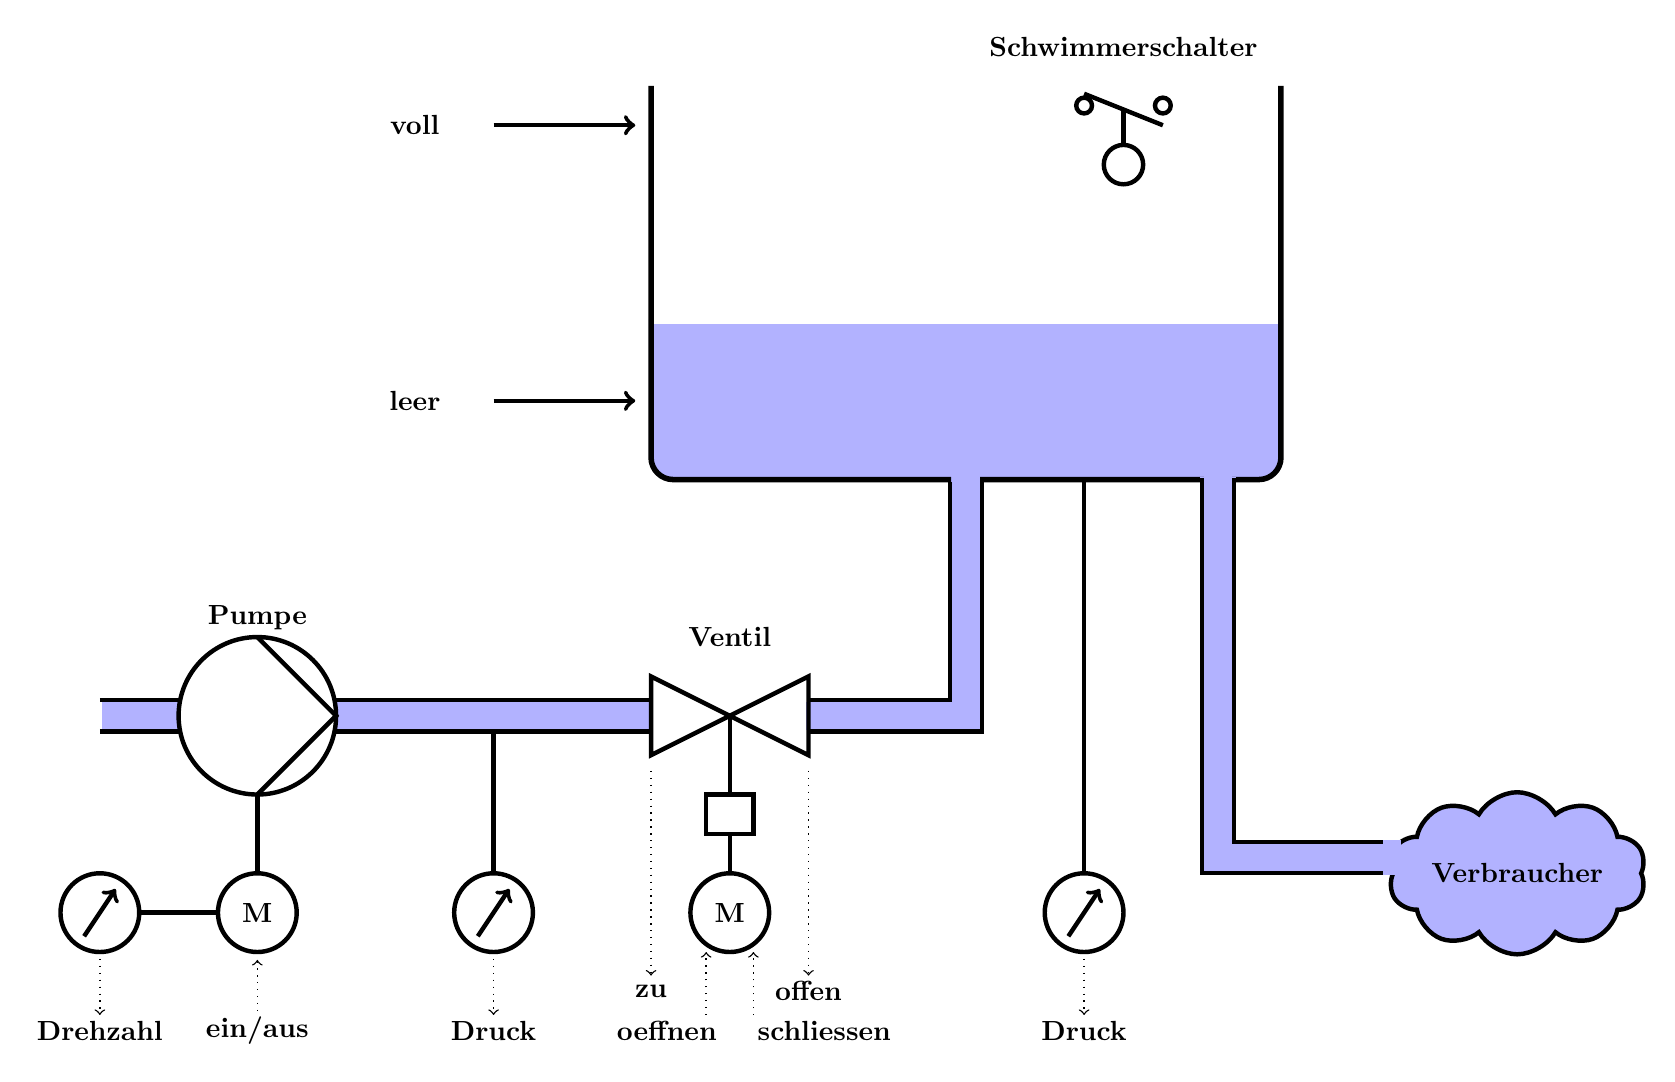
\begin{tikzpicture}
	
	\begin{scope}[ultra thick]
	
    %%%%%%%%%%%%%%%%%%%%%%%%%%%%%%%%%%%%%%%%%%%%%%%%%%%%%%%%%%%%%%%%%%%%%
    % Pumpe

    \filldraw[fill=blue!30, draw=blue!30] (-0.95,2.15) rectangle (6,1.85);
    \draw(-1,2.2) -- (6,2.2);
    \draw(-1,1.8) -- (6,1.8);
    
	\filldraw[color=white,draw=black] (1,2) circle (1cm);
	\draw(1,3) -- (2,2) -- (1,1);	
	\node at (1,3.25) {\bf Pumpe};

     %%%%%%%%%%%%%%%%%%%%%%%%%%%%%%%%%%%%%%%%%%%%%%%%%%%%%%%%%%%%%%%%%%%%% 
     % pumpenmotor
	\motor{1}{-0.5}
	\draw (1,-0) -- (1,1);
	
	\draw [<-,dotted, line width = 0.5pt] (1,-1.1) -- (1,-1.8);
	\node at (1,-2) {\bf ein/aus};

% Drehzahlmessung
   \draw(0.5,-0.5) -- (-0.5,-0.5);
   \messung{-1}{-0.5}
   	\draw [->,dotted,line width=0.5pt] (-1,-1) -- (-1,-1.8);
      \node at (-1,-2) {\bf Drehzahl};

% leitung zum Tank	
\filldraw[fill=blue!30, draw=blue!30] (8,2.15) rectangle (9.85,1.85);
\filldraw[fill=blue!30, draw=blue!30] (9.85,1.85) rectangle (10.15,5.1);
\draw(8,2.2) -- (9.8,2.2) -- (9.8,5);
\draw(8,1.8) -- (10.2,1.8) -- (10.2,5);
	
% Ventil	
	\ventil{7}{2}{Ventil}  % +-1 in x
	\draw [->,dotted,line width=0.5pt] (6,1.3) -- (6,-1.3);
	\node at (6,-1.5) {\bf zu};
    \draw [->,dotted,line width=0.5pt] (8,1.3) -- (8,-1.3);
	\node at (8,-1.5) {\bf offen};
%
% ventilmotor
	\motor{7}{-0.5}
    \draw (7,0.5) -- (7,-0);
    \draw [->,dotted,line width=0.5pt] (6.7,-1.8) -- (6.7,-1);
    \node at (6.2,-2) {\bf oeffnen};
    
    \draw [->,dotted,line width=0.5pt] (7.3,-1.8) -- (7.3,-1);
    \node at (8.2,-2) {\bf schliessen};

% primaerdruck
	\draw(4,1.8) -- (4,-0);
	\messung{4}{-0.5};
   	\draw [->,dotted,line width=0.5pt] (4,-1) -- (4,-1.8);
    \node at (4,-2) {\bf Druck};


% Tank
     \filldraw [draw=blue!30,fill=blue!30,rounded corners=8pt] (6,7.3) rectangle (14,5);
     % remove upper corners
     \filldraw[draw=white,fill=white] (6,7.5) rectangle ( 14,7);
     
	 \draw[line width=2pt,rounded corners=8pt](6,10) -- (6,5) -- (9.81,5);
	 \draw[line width=2pt, rounded corners = 8pt] (10.18,5) --(14,5) --  (14,10);
	 \draw (11.5,5) -- (11.5,0);
	 \messung{11.5}{-.5}
   	\draw [->,dotted,line width=0.5pt] (11.5,-1) -- (11.5,-1.8);
    \node at (11.5,-2) {\bf Druck};
%% Fuellstaende
    \node at (3,9.5) {\bf voll};
    \draw [->] (4,9.5) -- (5.8,9.5);
    \node at (3,6) {\bf leer};
    \draw [->] (4,6) -- (5.8,6);     
    

% auslauf
   	\filldraw[color=blue!30,draw=blue!30] (13.05,4.9) rectangle (13.35,6.1); % break hole
   	\node at (17,0) [cloud, fill=blue!30,draw,cloud puffs=10,cloud puff arc=120, aspect=2, inner ysep=1em] {\ \ \ \ \ \ \ \  \ \ \ \ \ \ \ \ \ \  } ;
   	\node at (17,0) {\bf Verbraucher};
   

   	\filldraw[color=blue!30,draw=blue!30] (13,5) rectangle (13.4,0);
   	\filldraw[color=blue!30,draw=blue!30] (13,0) rectangle (15.5,0.4);
   	
    \draw(13,5.02) -- (13,0) -- (15.3,0);
   	\draw(13.4,5.02) -- ( 13.4,0.4) -- (15.3,0.4);


        % Schwimmerschalter
       	\floatswitch{12}{9}

        
	\end{scope}
	

	\end{tikzpicture}
\end{document}